\documentclass[Main.tex]{subfiles} 
\begin{document}

\subsubsection{Komponent 5: Log}
Denne komponent fungerer som et f�lles loggingframework for hele systemet. Komponenten er implementeret via et singleton designpattern, hvilket sikrer, at det er den samme log der benyttes p� tv�rs af systemet. Den vigtigste funktion i komponenten er, at indskrive loggen i systemets database, men indeholder ogs� mulighed for at logge til fil, logge til et WPF-vindue og en log der bruges i simulerings�jemed. 
\\
Loggen er baseret p� et centralt interface, ILog, som indeholder funktionen logThis() og RobotMoved. Dette interface implementeres af forskellige klasser, der henholdsvis har til opgave at logge til forskellige medier. Dette betyder at logtypen kan udskiftes uden st�rre problemer, endda p� runtime.
Strukturen er fremvist p� billedet herunder:

\begin{figure}[H]
\centering
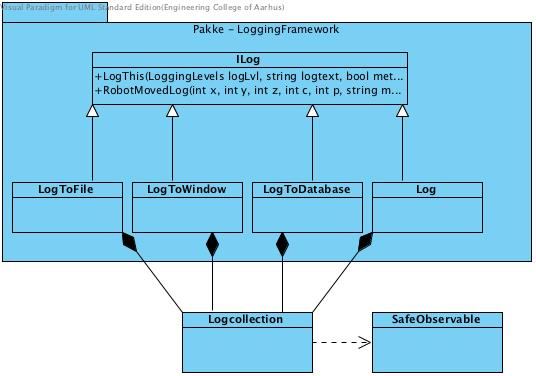
\includegraphics[scale=0.5]{Diagrammer/Klassediagrammer/Klassediagrammer/JPGFiler/Pakke_LogginFramework.jpg}
\caption{Sturktur over Log}
\end{figure}


Implementeringen af LogThis varierer fra logtype til logtype. Mens der altid logges et tidspunkt, et loglevel og en besked, er det ikke altid der logges f.eks. metoden eller filen hvorfra kaldet kommer. Metoden RobotMoved er en version af LogThis, som er specialiseret til at inds�tte beskeder om robottens bev�gelse.
Loggen er baseret p� et loglevel, defineret som en global enum, der indeholder alle loglevels.\\

\textbf{LogToFile}\\
Der gemmes her persistent til en fil p� disken. Filen gemmes som udgangspunkt i programmappen med et filnavn best�ende af logtidspunktet.\\

\textbf{LogToWindow}\\
En version, der logger til en collection, der implementerer INotifyPropertyChanged og derfor kan bindes til fra viewet\\

\textbf{LogToDB}\\
Den log der bruges under et normalt programforl�b, gemmer til databasen. Dette viste sig problemfyldt, da brugergr�nsefladen ikke kunne binde dertil. Derfor blev det valgt ogs� at opretholde en lokal kopi af loggen. Denne kopi skulle ydermere tilg�es af en tr�d anden end Dispatcher, hvilket ikke er muligt med en ObservableCollection, da denne ikke er tr�dsikker. Dette problem blev l�st ved at lave en klasse SafeObservable, som b�de implementerer INotifyPropertyChanged interfacet og indeholder tr�dbeskyttelse.




\end{document}